\documentclass[11pt]{article}

\usepackage[margin=1in]{geometry}
\usepackage{mathptmx} % Times New Roman 11pt
\usepackage{amsmath,amssymb,amsthm}
\usepackage{booktabs}
\usepackage{graphicx}
\usepackage{url}

\pagestyle{empty} % Geombinatorics requirement: no page numbers

\newtheorem{theorem}{Theorem}
\newtheorem{proposition}{Proposition}

\begin{document}

\begin{center}
{\fontsize{14}{17}\selectfont\bfseries Explicit Convex Polygon Bounds for Simple 8- and 9-Venn Diagrams\par}
\vspace{0.5em}
{\fontsize{12}{14}\selectfont Jinwon Kim\par}
\vspace{0.2em}
{\fontsize{11}{13}\selectfont Leeuwarden, The Netherlands \quad \texttt{[YOUR\_EMAIL\_HERE]}\par}
\end{center}

\vspace{0.8em}

\noindent\textbf{Abstract.}
Let $k^*(n)$ denote the minimum integer $k$ such that there exists a simple $n$-Venn diagram whose curves are all convex $k$-gons. While exact values are known for $n \le 7$, notably $k^*(6)=3$ and $k^*(7)=4$, to the best of our knowledge the best previously published explicit upper bounds for $n \ge 8$ remain $k^*(n) \le 2^{n-2}$ from Gr\"unbaum's inductive construction ($k^*(8) \le 64$ and $k^*(9) \le 128$), against the lower bounds $k^*(8) \ge 6$ and $k^*(9) \ge 8$ of Carroll, Ruskey, and Weston (2007). We establish the explicit upper bounds $k^*(8) \le 8$ and $k^*(9) \le 25$ via integer-lattice realizations in $[-589, 589]^2$ and $[-358651, 358651]^2$, respectively. For $n=9$, we overcome the crossing concentration of reducible lifts using a sliding-window CP-SAT wiring rebalancer paired with an unrestricted-angle inverse-radius linear program and dual-envelope angle ascent. Both realizations are certified in exact rational arithmetic and checked by standalone, dependency-free Lean~4 kernel proofs.

\section{Introduction}

A \emph{simple $n$-Venn diagram} is a family $\mathcal{C} = \{C_0, \dots, C_{n-1}\}$ of $n$ simple closed curves in $\mathbb{R}^2$ such that all intersections are transversal, at most two curves meet at any point, and each of the $2^n$ open regions $\bigcap_{i=0}^{n-1} X_i$ (where $X_i$ is either the bounded interior or unbounded exterior of $C_i$) is nonempty and connected. By Euler's formula, the induced $4$-regular plane graph has $V = 2^n - 2$ vertices, $E = 2^{n+1} - 4$ edges, and $F = 2^n$ faces.

Let $k^*(n)$ be the smallest integer $k$ for which a simple $n$-Venn diagram exists with every curve $C_i$ a convex $k$-gon. Carroll, Ruskey, and Weston~\cite{CRW2007} proved the general lower bound
\[
k^*(n) \ge \left\lceil \frac{2^n - 2 - n}{n(n-2)} \right\rceil
\]
and settled $k^*(7) = 4$ with a simple symmetric $7$-Venn diagram of convex quadrilaterals, following Carroll's resolution of $k^*(6) = 3$~\cite{Carroll2000}. For $n=8$ and $n=9$, this lower bound gives $k^*(8) \ge 6$ and $k^*(9) \ge 8$. On the upper-bound side, to the best of our knowledge the best previously published explicit upper bounds for $n \ge 8$ remain $k^*(n) \le 2^{n-2}$ from Gr\"unbaum's inductive convex construction~\cite{Grunbaum1975}, which gives $k^*(8) \le 64$ and $k^*(9) \le 128$ (see Table~1 of~\cite{CRW2007} and~\cite{Grunbaum1992,RuskeyWeston2005}). In this note we improve both explicit upper bounds.

\begin{theorem}\label{thm:main}
There exists a simple convex $8$-Venn diagram consisting of eight strictly convex octagons with integer vertices in $[-589, 589]^2$, and a simple convex $9$-Venn diagram consisting of nine strictly convex $25$-gons with integer vertices in $[-358651, 358651]^2$. Consequently,
\[
6 \le k^*(8) \le 8 \qquad \text{and} \qquad 8 \le k^*(9) \le 25.
\]
\end{theorem}

\begin{table}[h]
\centering
\small
\begin{tabular}{@{}cccccc@{}}
\toprule
$n$ & Lower Bound~\cite{CRW2007} & Previous UB~\cite{Grunbaum1975} & \textbf{New UB} & Lattice Box & Max Pairwise Crossings \\
\midrule
$6$ & $3$ & $3$~\cite{Carroll2000} & --- & --- & --- \\
$7$ & $4$ & $4$~\cite{CRW2007} & --- & --- & --- \\
$8$ & $6$ & $64$  & $\mathbf{8}$  & $[-589, 589]^2$       & $14$ \\
$9$ & $8$ & $128$ & $\mathbf{25}$ & $[-358651, 358651]^2$ & $22$ \\
\bottomrule
\end{tabular}
\caption{Known bounds and new certified realizations for simple convex $n$-Venn diagrams.}
\label{tab:summary}
\end{table}

\section{Monotone Wirings, Piercing Lower Bounds, and CP-SAT Rebalancing}

By the characterization of Bultena, Gr\"unbaum, and Ruskey~\cite{BGR1999}, a family of finitely intersecting simple closed curves admits a convex drawing if and only if it is \emph{monotone}. Choosing an origin $O$ in the nonempty common interior $\bigcap_{i=0}^{n-1} \operatorname{int}(C_i)$, every ray from $O$ crosses each convex boundary $C_i$ in a unique point. Sweeping a ray counterclockwise around $O$ records a cyclic sequence of $M = 2^n - 2$ adjacent transpositions (a \emph{monotone wiring}) on the radial permutation $\pi_t$ of the $n$ curves.

Any monotone wiring imposes an exact combinatorial lower bound on the number of sides of each curve $C_c$. Whenever $C_c$ exits the interior of another curve $C_o$ at swap $t_{\text{out}}$ and next re-enters $C_o$ at swap $t_{\text{in}}$, convexity of $C_o$ forbids a single straight side of $C_c$ from spanning the entire cyclic interval $[t_{\text{out}}+1, t_{\text{in}}] \pmod M$. Thus the corner indices of $C_c$ must hit every such outside-arc over $o \ne c$. The minimum cardinality of a hitting set—the \emph{circular-arc piercing lower bound} $\operatorname{plb}(C_c)$—is computable exactly and satisfies $|V(C_c)| \ge \operatorname{plb}(C_c)$.

Rather than searching directly in unconstrained vertex coordinates, our reverse-direction pipeline begins from a valid monotone wiring with guaranteed topology ($V = 2^n - 2$, $F = 2^n$) and iteratively eliminates polygon corners while locking the radial swap order. For $n=8$, polar-coordinate compression combined with topology-locked vertex collapse and cell inflation reduced an initial monotone $8$-Venn wiring down to eight strictly convex octagons, subsequently quantized to $[-589, 589]^2$ (listed explicitly in the Appendix).

Extending this approach to $n=9$ encounters a sharp combinatorial barrier when lifting an $8$-Venn diagram by adding a ninth curve:

\begin{proposition}\label{prop:reducible}
In any simple convex $9$-Venn diagram of $k$-gons obtained as a reducible lift of an $8$-Venn diagram (where $C_8$ bisects all $256$ faces), the ninth curve has degree $256$ and satisfies $k \ge 16$.
\end{proposition}
\begin{proof}
To bisect all $2^8 = 256$ faces of the $8$-Venn subdiagram, $C_8$ must cross the other eight curves $256$ times in total. By averaging, at least one pair $(C_8, C_o)$ intersects at least $256 / 8 = 32$ times. Since two convex $k$-gons intersect transversally in at most $2k$ points, $2k \ge 32$, so $k \ge 16$.
\end{proof}

Lifting our certified $8$-Venn wiring to $n=9$ via CP-SAT yielded a reducible $510$-swap wiring with maximum degree $256$, maximum pairwise crossings $34$, and exact piercing profile $\operatorname{plb} = [17, 17, 13, 16, 14, 17, 17, 17, 35]$. Geometric compression on this reducible wiring reached uniform $36$-gons and could not pass the combinatorial floor $35$ on $C_8$.

To break this bottleneck, we applied a sliding-window CP-SAT rebalancer over contiguous windows of $W \in [30, 62]$ consecutive swaps. Inside each window, the boundary permutations $\pi_{\text{start}}, \pi_{\text{end}}$ and the exact set of $W$ region bitmasks created within the window are preserved via a bijection, while the internal swap order is re-optimized to minimize a quadratic-weighted degree objective. Across multiscale passes, crossings shifted off $C_8$ onto $C_0, \dots, C_7$:
\begin{itemize}
\item Maximum curve degree fell from $256$ to $142$ (profile $[114, 102, 102, 104, 92, 116, 112, 136, 142]$).
\item Maximum pairwise crossings fell from $34$ to $22$ (strictly below the reducible-lift floor $32$).
\item Maximum piercing lower bound fell from $35$ to $17$ (profile $[17, 14, 13, 16, 12, 15, 15, 16, 15]$).
\end{itemize}

\section{Inverse-Radius LP Compression}

Fix checkpoint ray angles $0 \le \theta_0 < \dots < \theta_{M-1} < 2\pi$ and a subset of corner indices $I_c \subset \{0, \dots, M-1\}$ for each curve $C_c$. In inverse-radius coordinates $u_{c,j} = 1 / r_{c,j} > 0$, both strict convexity and checkpoint radial ordering become strictly linear in $u$:
\begin{enumerate}
\item For any three consecutive corners with single-edge angular gaps $0 < \Delta_1, \Delta_2 < \pi$, strict counterclockwise turning is equivalent to
\[
\frac{u_{\text{prev}} \sin\Delta_2 + u_{\text{next}} \sin\Delta_1 - u_{\text{cur}} \sin(\Delta_1 + \Delta_2)}{\sin\Delta_1 + \sin\Delta_2} \ge \tau.
\]
\item Along each ray $\theta_t$, $u_c(\theta_t)$ is a linear combination of the two bracketing corners of $C_c$, yielding linear separation constraints $u_{\pi_t(r)}(\theta_t) - u_{\pi_t(r+1)}(\theta_t) \ge \tau$.
\end{enumerate}

Maximizing $\tau$ is a sparse linear program, and by Danskin's envelope theorem its dual multipliers provide an exact subgradient $\nabla_\theta \tau^*$ for projected gradient ascent on the angle simplex. Starting from trivial $510$-gons on the rebalanced irreducible $9$-Venn wiring, iterative batch thinning, single-vertex drops, $2$-to-$1$ midpoint merges, and parallel pinned-spread angle rescues compressed the curves to side counts $[24, 24, 24, 25, 23, 25, 24, 24, 24]$. Padding to nine uniform $25$-gons, inflating $\tau$, and binary-searching the smallest valid integer lattice scale yielded the certified realization in $[-358651, 358651]^2$.

For $n=8$, our certified octagon realization has degree profile $[62, 62, 62, 68, 58, 62, 58, 76]$, maximum pairwise crossings $14$, and piercing lower bound $\operatorname{plb} = [7, 7, 7, 8, 7, 7, 7, 8]$. Targeted CP-SAT searches encoding the circular-arc piercing automaton directly inside local windows up to $W=68$ did not reduce $\max_c \operatorname{plb}(C_c)$ below $8$; resolving whether $k^*(8)$ equals $6$, $7$, or $8$ remains an open problem.

\section{Exact Arithmetic and Lean 4 Formal Certification}

Because floating-point realizations near tight margins can conceal degenerate contacts or missing microscopic faces, both lattice constructions are independently verified in exact rational arithmetic (Python \texttt{fractions.Fraction}) and by standalone Lean~4 kernel proofs (\texttt{SimpleConvex8VennK8.lean} and \texttt{SimpleConvex9VennK25.lean}) using zero external libraries, zero \texttt{sorry}, and zero \texttt{native\_decide}. By definitional kernel reduction (\texttt{by decide}), Lean~4 certifies four finite integer predicates:
\begin{enumerate}
\item \emph{Simple strict convexity (winding number $1$):} For every directed edge $(v_i, v_{(i+1)\bmod K})$ of every polygon, all $K-2$ non-incident vertices $v_j$ ($j \notin \{i, (i+1)\bmod K\}$) satisfy strictly positive orientation $\operatorname{orient}(v_i, v_{(i+1)\bmod K}, v_j) > 0$. This excludes duplicate vertices and self-intersecting star polygons (winding number $\ge 2$): every directed edge is a counterclockwise edge of the convex hull $\operatorname{conv}\{v_0,\dots,v_{K-1}\}$, forcing the cyclic sequence to traverse the convex hull boundary exactly once.
\item \emph{Simplicity and graph connectivity:} Across all $\binom{n}{2} K^2$ edge pairs, zero degenerate contacts occur, every curve pair intersects transversally at least twice, and the total crossing count equals exactly $V = 2^n - 2$ ($254$ for $n=8$, $510$ for $n=9$).
\item \emph{Zero triple points:} An explicit list of $V$ transversal edge-pair crossings is verified to be strictly increasing in exact rational lexicographical order, proving all $V$ intersection points are pairwise distinct.
\item \emph{Bijective subset witnessing:} Indexed sequentially over all $m = 0, 1, \dots, 2^n - 1$ (ruling out duplicate bitmasks), each explicit rational witness point lies strictly inside every polygon with bit $1$ and strictly outside every polygon with bit $0$ (via an explicit separating edge).
\end{enumerate}

By the Jordan Curve Theorem, the arrangement forms a connected $4$-regular plane graph with $V = 2^n - 2$ and $E = 2V$, so Euler's formula gives exactly $F = E - V + 2 = 2^n$ faces. Since points with distinct containment bitmasks cannot lie in the same face, the $2^n$ strictly separated witnesses force a bijection between faces and subsets of $\{0, \dots, n-1\}$ by the Pigeonhole Principle, proving that all $2^n$ Venn regions are nonempty and connected.

\begin{figure}[h]
\centering
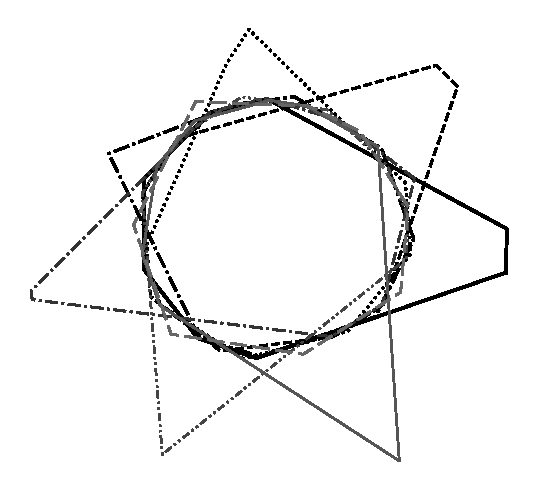
\includegraphics[width=0.47\textwidth]{fig1_8venn_bw.pdf}\hfill
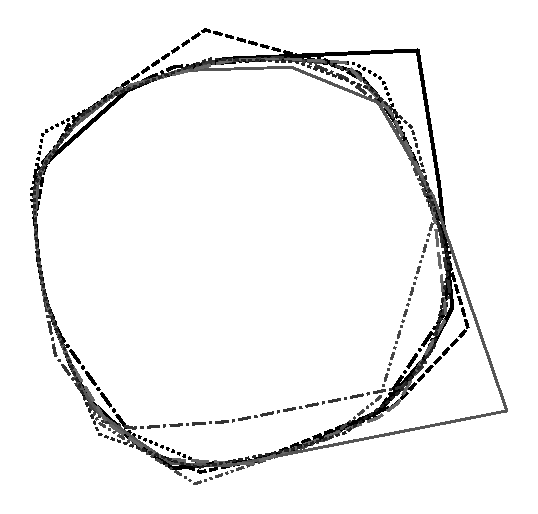
\includegraphics[width=0.47\textwidth]{fig2_9venn_bw.pdf}
\caption{Certified simple convex Venn diagrams: (left) $n=8$ with eight octagons in $[-589, 589]^2$; (right) $n=9$ with nine uniform $25$-gons in $[-358651, 358651]^2$.}
\label{fig:diagrams}
\end{figure}

\section*{Appendix: Integer Vertices for the $n=8$ Octagon Diagram}

Table~\ref{tab:coords8} lists all $64$ integer vertices of the eight strictly convex octagons in $[-589, 589]^2$ in counterclockwise order. Complete witness coordinates, all $225$ integer vertices for the $n=9$ uniform $25$-gon realization, independent Python $\mathbb{Q}^2$ verifiers, and standalone Lean~4 kernel certificates are archived at \url{https://github.com/Gelukkig95/simple-convex-venn} (Zenodo DOI: \url{https://doi.org/10.5281/zenodo.24572392}).

\begin{table}[h]
\centering
\footnotesize
\begin{tabular}{@{}cl@{}}
\toprule
Curve & Counterclockwise Integer Vertices $(x,y) \in [-589, 589]^2$ \\
\midrule
$C_0$ & $(497,-152),\; (499,-52),\; (-49,245),\; (-178,215)$ \\
        & $(-330,64),\; (-332,-144),\; (-208,-302),\; (-74,-348)$ \\[2pt]
$C_1$ & $(386,273),\; (337,322),\; (-254,155),\; (-334,30)$ \\
        & $(-316,-207),\; (-157,-331),\; (99,-300),\; (215,-227)$ \\[2pt]
$C_2$ & $(267,53),\; (-91,404),\; (-141,328),\; (-334,-108)$ \\
        & $(-294,-226),\; (-104,-349),\; (135,-287),\; (279,-110)$ \\[2pt]
$C_3$ & $(286,-75),\; (212,132),\; (13,250),\; (-113,234)$ \\
        & $(-412,120),\; (-204,-302),\; (-66,-344),\; (199,-253)$ \\[2pt]
$C_4$ & $(288,63),\; (116,196),\; (-51,246),\; (-179,216)$ \\
        & $(-589,-194),\; (-587,-214),\; (97,-299),\; (214,-225)$ \\[2pt]
$C_5$ & $(272,-22),\; (226,91),\; (89,220),\; (-107,250)$ \\
        & $(-256,154),\; (-335,30),\; (-289,-568),\; (270,-120)$ \\[2pt]
$C_6$ & $(204,136),\; (40,229),\; (-43,242),\; (-215,195)$ \\
        & $(-301,93),\; (-335,-110),\; (-295,-227),\; (253,-583)$ \\[2pt]
$C_7$ & $(273,-1),\; (163,171),\; (45,229),\; (-213,239)$ \\
        & $(-355,-43),\; (-269,-293),\; (33,-339),\; (256,-197)$ \\[2pt]
\bottomrule
\end{tabular}
\caption{Exact integer vertices of the certified simple convex $8$-Venn diagram of eight octagons.}
\label{tab:coords8}
\end{table}

\begin{thebibliography}{9}
\bibitem{BGR1999}
B.~Bultena, B.~Gr\"unbaum, and F.~Ruskey,
\emph{Convex drawings of intersecting families of simple closed curves},
Proc.\ 11th Canadian Conference on Computational Geometry (CCCG), 1999.

\bibitem{Carroll2000}
J.~Carroll,
\emph{Drawing Venn triangles},
Technical Report HPL-2000-73, Hewlett-Packard Laboratories, Bristol, 2000.

\bibitem{CRW2007}
J.~Carroll, F.~Ruskey, and M.~Weston,
\emph{Which $n$-Venn diagrams can be drawn with convex $k$-gons?},
Discrete \& Computational Geometry \textbf{37}(4) (2007), 619--628.

\bibitem{Grunbaum1975}
B.~Gr\"unbaum,
\emph{Venn diagrams and independent families of sets},
Mathematics Magazine \textbf{48} (1975), 12--23.

\bibitem{Grunbaum1992}
B.~Gr\"unbaum,
\emph{Venn diagrams II},
Geombinatorics \textbf{2} (1992), 25--31.

\bibitem{RuskeyWeston2005}
F.~Ruskey and M.~Weston,
\emph{A survey of Venn diagrams},
Electronic Journal of Combinatorics, Dynamic Survey \textbf{DS5} (2005).
\end{thebibliography}

\end{document}
